\documentclass[11pt,a4paper]{report}
 %use Times
\usepackage{times}
% For figuresez
\usepackage{graphicx} % more modern
%\usepackage{epsfig} % less modern
\usepackage{subfigure} 

% For citations
\usepackage{natbib}

% For algorithms
\usepackage{algorithm}
\usepackage{algorithmic}



%custom packages
\usepackage{amssymb,amsmath}
\usepackage{amsthm}
\usepackage[usenames,dvipsnames]{xcolor}
\usepackage{enumitem}

%custom theorems 
\newtheorem{definition}{Definition}
\newtheorem{lemma}{Lemma}
\newtheorem{Theorem}{Theorem}
\newtheorem{example}{Example}
\newtheorem{statement}{Statement}
\newtheorem{corollary}{Corollary}
\begin{document}




Hi,
\\
\\
I have computed histograms for MMD under various settings, see the Figure below.

Let
$$\Sigma = \left( \begin{array}{cc} 15.5&14.5\\ 14.5&15.5 \end{array} \right),$$
$P_0 = N([0 \quad 0],\Sigma)$, $P_1 = N([0 \quad 1],\Sigma)$ and $P_6 = N([0 \quad 6],\Sigma)$. 

The top graph compares MMD estimator distribution calculated using samples from $(P_0,P_0)$ and $(P_0,P_6)$ i.e. $MMD(P_0,P_0)$ and $MMD(P_0,P_6)$. \textbf{The samples were obtained from Gibbs sampler, size of each sample was 200}. We see that the histograms are disjoint so we would expect test procedures to have $5\%$ type one error and $0\%$ type two error.

The wild bootstrap reports $17 \%$ type one error (I believe this is  due to  'artificial degeneration' which does not converge very well) and $0\%$ type two error. 

Middle graph compares MMD estimator distribution calculated using samples from $(P_0,P_0)$ and $(P_0,P_1)$ i.e. $MMD(P_0,P_0)$ and $MMD(P_0,P1)$. The samples were also obtained form the Gibbs sampler. $95$ percentile  of the $MMD(P_0,P_0)$ distribution is 25.55. Empirical probability that  $MMD(P_0,P1)$ estimator is smaller then 25.55 is 0.93. Therefore we expect type two error to be around $93\%$.

Finally the bottom graph  compares MMD estimator distribution calculated using samples from $(P_0,P_0)$ and $(P_0,P_1)$, but the samples have no temporal dependence (they are IID, generated using Matlb function for multivariate Gaussian).  \textbf{ In this setting the expected type two error is $14 \%$ !}. This is  inconsistent with the result obtained by Dino - he reported type two error around $1\%$. That means we have different MMD procedures or there is something going on with random variables generation (e.g. mistake in $\Sigma$ ) or some other bug. 

All histograms were obtained from 2000 samples.   

\begin{figure}
\centering  
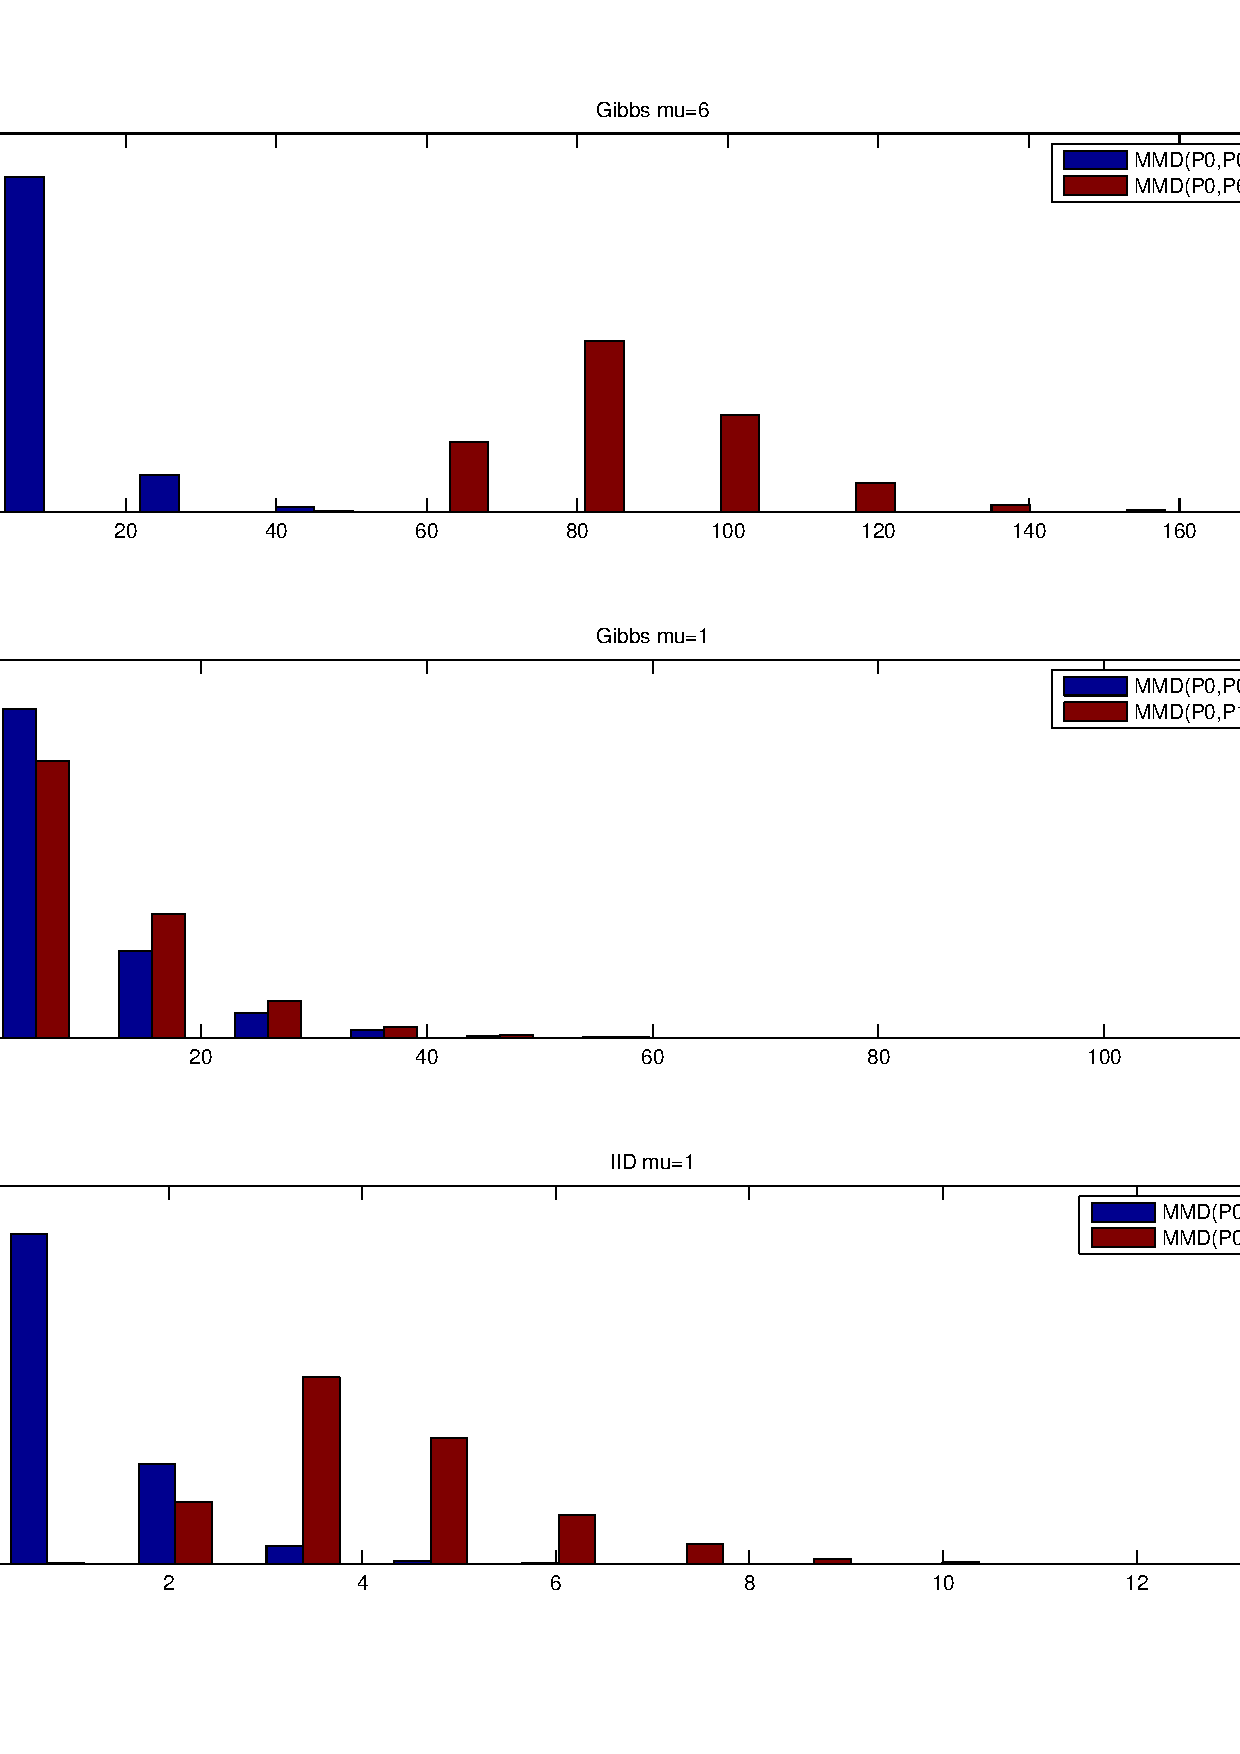
\includegraphics[width=1.4\textwidth]{histograms.pdf}
\label{hist}
\end{figure}
\end{document}